\makeatletter
\newcommand*{\l@code}{\l@figure}
\newcommand*{\listofcode}{ %
  \begin{singlespace}
  \clearpage
  \null
  \vskip 0.4in
  \center{LIST OF SAMPLE CODE} \\
  \vskip 4\lineheight
  \@starttoc{cod}
  \end{singlespace}
}
\makeatother
\begin{document}
  \frontmatter
  \clearpage
  \parskip 7.2pt
  
  \chapter*{}
  \begin{singlespace}
    \addcontentsline{toc}{chapter}{Abstract}
    \vspace{-1in}
    \center{ABSTRACT}
    
    \vspace{2\lineheight}
    PSODASCRIPT: APPLYING ADVANCED LANGUAGE CONSTRUCTS TO OPEN-SOURCE PHYLOGENETIC SEARCH
    
    \vspace{1.5\lineheight}
    \begin{center}
      Adam R. Teichert \\
      \vspace{\lineheight}
      
      Department of Computer Science \\
      \vspace{\lineheight}
      
      Bachelor of Science \\
    \end{center}
    
    \vspace{1.5\lineheight}
  \end{singlespace}
  Phylogenetic inference may be approached as a search through phylogenetic tree space to find, from molecular data such as DNA, a likely evolutionary tree connecting a group of organisms.
  For reasonable sized data sets, however, the vastness of this space makes an exhaustive search impractical, so most popular phylogenetic analysis software packages use heuristic searches to narrow down the tree space in order to arrive at a solution without analyzing every possible tree for a given data set.
  Unfortunately, such heuristic searches can get stuck in local optima preventing the search from arriving at the globally optimal solution.
  Often, stagnation in local optima can be avoided by combining a variety of heuristic searches and parameter settings into meta-searches.
  Advanced language constructs in an open-source phylogenetic analysis package allow researchers to better exploit and explore the domain of phylogenetic meta-searches.
  The work involved in designing and implementing PsodaScript---an internal scripting language for BYU's open-source phylogenetic analysis package, PSODA---has become a culminating experience of my undergraduate education.
  
  \chapter*{}
  \begin{singlespace}
  \addcontentsline{toc}{chapter}{Acknowledgments}
  \vspace{-1in}
  \center{ACKNOWLEDGMENTS}
  
  \vspace{1.5\lineheight}
  \end{singlespace}
  Special thanks go to Jonathan Krein, my partner on the great majority of this project and the initial impetus to my involvement in the project, whose persistence and concern for quality were truly inspirational.
  I also thank Dr. Quinn Snell, my adviser, who has gone out of his way to provide me with many important experiences that have molded my outlook on my future profession.
  Dr. Mark J. Clement has provided significant support in the development of this honors thesis.
  I also thank Hyrum Carroll and other members of the Computational Science Laboratory for their patience and assistance, including Kenneth Sundberg, whose continuing interest in and improvement to the PSODA code base give me hope that this work will not be soon forgotten.
  
  \pagebreak

  \clearpage
  \setlength{\cftbeforetoctitleskip}{0.4in}
  \setlength{\cftaftertoctitleskip}{0.5\lineheight}
  \setlength{\cftbeforeloftitleskip}{0.4in}
  \setlength{\cftbeforelottitleskip}{0.4in}
 
  \setlength{\cftchapindent}{0.0em}
  \setlength{\cftsecindent}{0.0em}
  \setlength{\cftsubsecindent}{0.0em}
  \setlength{\cftsubsubsecindent}{0.0em}

  \renewcommand{\cfttoctitlefont}{\hfill\textnormal\normalsize}
  \renewcommand{\cftloftitlefont}{\hfill\textnormal\normalsize}
  \renewcommand{\cftlottitlefont}{\hfill\textnormal\normalsize}

  \renewcommand{\cftaftertoctitle}{\hfill}
  \renewcommand{\cftafterloftitle}{\hfill}
  \renewcommand{\cftafterlottitle}{\hfill}

  \renewcommand{\cftchapleader}{\cftdotfill{\cftdotsep}}
  \renewcommand{\contentsname}{TABLE OF CONTENTS}
  \renewcommand{\listfigurename}{LIST OF FIGURES}
  \renewcommand{\listtablename}{LIST OF TABLES}

  \tableofcontents
  \clearpage
  \listoffigures
  \clearpage
  \listoftables
  \clearpage
  \listofcode %{\hfill\textnormal\normalsize{LIST OF CODE SAMPLES}\hfill}

  \mainmatter
  
  \chapter{Introduction}
  Infection with the Human Immunodeficiency Virus (HIV\index{HIV}) is a precursor to the Acquired Immune Deficiency Syndrome (AIDS\index{AIDS}).
  In the year 2007 alone, an estimated 2.5 million people were newly infected with HIV while an estimated 2.1 million people died of AIDS \cite{unaids2006aeu}.
  In 2004, researchers showed that documenting the overall evolution of the HIV virus is crucial to the development of successful vaccines \cite{Rambaut}.
  Phylogenies\index{phylogeny} are essential tools for understanding evolutionary and genetic relationships \cite{Felsenstein}.
  Just as a pedigree chart represents an individual's ancestral tree, a phylogeny is a tree that represents the evolutionary connections among organisms.
  Phylogenetic trees can be inferred through analysis of genetic information such as that contained in DNA sequences.
  However, the vastness of phylogenetic tree space---the sheer number of possible phylogenetic trees that could connect a given group of organisms---leaves analysis software with an enormous challenge in terms of computational time complexity even for data sets of only a few hundred taxa.
  Because of this computational challenge, phylogenetic inference often relies on heuristic based searches to avoid an exhaustive search of all possible trees.
  
  In order to narrow the search space and arrive more efficiently at a solution, heuristic searches make assumptions about which areas of the space are more likely to contain the best answer.
  Unfortunately if these assumptions are not absolutely correct, such searches may rule out, and thus leave unexplored, the area of the search space that contains the truly optimal solution, thus getting stuck in a local optimum.
  More robust algorithms called meta-searches attempt to avoid stagnation in local optima by combining multiple heuristic searches.
  Implementing advanced language constructs in an open-source phylogenetic analysis package provides researchers with a framework for exploiting already discovered meta-searching algorithms as well as exploring other approaches.
  The result of these implementation efforts is the internal scripting language, PsodaScript.

  While the bulk of my efforts in the project are found in the actual design and implementation, this written thesis documents the development of PsodaScript.
  Chapter two reviews the concepts and work that have served as the background and foundation of the project.
  Chapter three provides an overview of the design and implementation of PsodaScript.
  Chapter four presents a few areas for future work with PsodaScript, and Chapter 5 highlights some of the personal benefits I gained from participation in the project.
  Appendix A contains a guide to PsodaScript syntax and semantics.
  Appendix B includes some sample PsodaScript program blocks.
  
  \chapter{From Phylogenetics to PAUP to PsodaScript}
  In this chapter, I present the fundamental concepts and foundational efforts upon which PsodaScript was created.
  First, I review briefly the topics of phylogenetics, meta-searching, and the role of internal scripting in phylogenetic inference.
  I then provide an overview of several products related to PsodaScript and their relevance to this project.

  \section{Phylogenetics}
  Phylogenetics is the study of genetic relationships among species.
  Researchers often describe these relationships with phylogenetic trees, which can be inferred from molecular data using methods such as parsimony or maximum likelihood with the aim to place more closely related organisms closer to each other on the tree.
  Phylogenetic researchers seek to find trees that represent the most accurate view of phylogenetic relationships.

  Interest in phylogenetic research over the past few decades has led to the creation of several phylogenetic inference software packages.
  Inferring a likely phylogenetic tree involves a search through phylogenetic tree space---looking for the tree with the best score based on some fitness metric (such as parsimony).
  Unfortunately, since the phylogenetic inference problem has been proven to be NP-complete \cite{Graham}, for large---or even moderately sized---data sets, an exhaustive search of this nature cannot be completed in reasonable time.

  Heuristic searches are an alternative to exhaustive searches.
  Although heuristic searches can greatly narrow the search space, and thus achieve fairly good results in a more reasonable amount of time, they often cannot guarantee that their solution is optimal with respect to the desired criteria.
  Since heuristic searches disregard certain paths in the search space as they seek an optimal solution, they may end up finding a local optimum that is worse than the global optimum.

  \section{Meta-searching}
  In an effort to avoid local optimum traps, researchers have experimented with methods for combining various heuristic searches into a single meta-search.

  Phylogenetic packages can facilitate meta-searching in three basic ways:

  \begin{enumerate}
  \item{{\emph{Package Modification}}---The software package itself may be modified and recompiled to introduce a new meta-search.}
  \item{{\emph{External Wrappers}}---External applications or scripts may serve as wrappers to call already existing functionality and construct meta-searches.}
  \item{{\emph{Internal Scripting}}---An internal scripting language may be incorporated into the package to allow the user to specify how to combine existing functionality into meta-searches.}
  \end{enumerate}
  
  \subsection{Package Modification}
  One approach to combining existing heuristic search implementations into meta-searches is to implement the meta-search as an additional built-in part of the software package, calling existing methods and using the implementation language to orchestrate the interaction between parts of the meta-search.
  One caveat connected with this method, of course, is that researchers may not have access to the source code, since the source code of some of the most popular packages is not publicly available.
  Furthermore, even with available source code, without a carefully designed architecture, seemingly small extensions to large software products can require extensive modifications, making extension even less practical.
  Changes to the software code base also require compilation which may be time consuming and cumbersome for large projects.
  Finally, extension in this way requires some understanding of the existing code as well as competence in the implementation programming language.

  \subsection{External Wrappers}
  An alternative to package modification is to use external programs or scripts to combine built-in functionality.
  DCM \cite{Roshan} is one example of such an approach.
  The DCM program divides a phylogenetic inference problem into sub tasks which it delegates to existing programs.
  Another example of this method would be the use of shell scripting to execute command-line runnable programs to perform a meta-search.
  Perl, a scripting language that is especially suited for easily implementing text manipulation applications, could also be used to call other programs and to perform data manipulation.
  Constructing meta-searches using existing programs wrapped with scripts has the advantage of being widely available.
  Unfortunately, such wrapper programs significantly increase the complexity and decrease the clarity of meta-search algorithms which could hinder the exploration of better meta-search algorithms.
  
  \subsection{Internal Scripting}
  A third approach to meta-search construction requires that the package provide an internal scripting language which can be used by researchers to describe meta-search algorithms in terms of built-in commands and constructs.
  Depending on the extent of scripting features available in the product, this approach can give power and flexibility to researchers without overly increasing the complexity of the meta-search description.
  A variety of scripting capabilities exist in current phylogenetic packages.
  In the following section, I review scripting possibilities in a few of these packages.

  \section{Meta-searching in Current Software Packages}
  Phylip \cite{Phylip} is one of the longest maintained phylogenetic packages.
  It consists of a collection of command-line executed programs written in C that can serve as a toolbox for carrying out phylogenetic analysis.
  Although significantly slower than most other popular packages, Phylip is fairly simple to install and execute.
  Phylip is also open source but has no internal interpreter or scripting capabilities.

  Programs such as Poy \cite{Poy} and PAUP* \cite{PAUP} provide a very limited internal scripting language, with basic commands that can be run sequentially.
  Some tools have been created that produce large input files to PAUP* in order to simulate a loop.

  BioPerl \cite{Stajich} is a collection of Perl modules that are useful in manipulating text to provide conversions between the output of one program to the format needed for input into another; however, BioPerl is ill suited to carry out elaborate meta-searches.
  Perl, an interpreted language, is relatively slow compared to compiled languages such as C.
  Also, the syntax of Perl can be an obstacle to newcomers.

  TNT \cite{TNT} has become a pace setter among phylogenetic software tools, achieving excellent phylogenetic search speeds on large (200-1000 taxa \cite{goloboff1999ald}) data sets and pioneering internal scripting in phylogenetic packages.
  TNT's source code, however, is proprietary and currently only facilitates parsimony methods.

  Because of the success of PAUP* as well as the proprietary restrictions that limit it, researchers at BYU began the development of an open-source alternative package, known as Phylogenetic Search Open-source Data Analysis (PSODA) \cite{PSODA}.
  For several tasks, PSODA is becoming a viable alternative to both open-source and proprietary phylogenetic packages.
  Modeled after PAUP*, however, PSODA has suffered from the same scripting shortcomings as PAUP*.
  The following section elaborates on these shortcomings.

  \section{The Goals of PsodaScript}
  Before the implementation of PsodaScript, an input file in PSODA (as in PAUP*) contained a program block---known as the PAUP block---which consisting of a number of command calls with various parameter settings.
  PSODA had a basic interpreter to execute the program blocks, but the PSODA interpreter needed some non-trivial adjustments to facilitate our goals of implementing an enhanced scripting language (Chapter \ref{chp:implementation} details these adjustments).
  The language---known as PsodaScript---as well as the mechanism we were designing to execute PsodaScript programs would need to meet several goals which I outline in this section.

  First, to facilitate integration of PSODA into the bioinformatics field, PsodaScript needed to be easy for researchers, and particularly PAUP* users, to adopt.
  By making PsodaScript's syntax compatible with existing PAUP* syntax, PAUP* users would be able to smoothly make the transition to PSODA and to begin to take advantage of PsodaScript's advanced features.

  Also, in order to better facilitate meta-search exploration and exploitation, PsodaScript would need to add several language constructs that would surpass the basic command-list programming available in PAUP*.
  The following chapter describes these constructs.

  While adding increased functionality, however, we would also need to make an effort to ensure that the syntax introduced by these advanced features could be easily learned and used by people with a limited programming background.

  Finally, the language needed to be designed and implemented in a way that would facilitate maintenance and future extension.

  \chapter{PsodaScript Design and Implementation}
  \label{chp:implementation}
  The tasks involved in embedding a full-fledged interpreted programming language into the previously existing architecture of PSODA can be divided into five main categories:

  \begin{enumerate}
    \item{The PSODA Program Graph}
    \item{Variables and Expressions}
    \item{Variable Environments and Scoping}
    \item{User-Defined Commands}
    \item{Error Checking}
  \end{enumerate}

%  As we began work on our task of converting the feeble scripting features available in PSODA into a fully fledged scripting language, several things remained unclear and daunting.
%  I was new to the PSODA project, I had never used tools to generate parsers or lexical analyzers, and the domain of phylogenetic research was completely foreign to me.
%  The design and implementation involved in the project would evolve iteratively and would involve several course corrections as we became increasingly better qualified to recognize implications of our decisions with regard to the goals of our project.

  In this chapter, I present a description of the design and implementation relating to each of these categories.

  \section{The PSODA Program Graph}
%  The first few days of work, involved exploration of the existing project code.
%  As we became familiar with the various parts of the software system, we turned our attention towards completion of our first subtask.
  The first significant task required a substantial reworking of the PSODA framework to lay the foundation for incorporating advanced language constructs.
  Before work had begun on the PsodaScript project, the parser had been responsible for calling methods of the interpreter as commands were parsed from the input file.
  Since the parser stepped through the input file in a sequential manner, loops and conditionals were impractical if not impossible.
  In order to add these and other programming constructs, we would need to modify the parser in such a way that, at parse time, a graph---representing the structure of the program---would be produced that could then be navigated and executed without being consumed.
  As the graph executed, the state of the program would be updated, controlling the flow of execution.

  My partner and I spent several days contemplating and experimenting with various ways to represent the program as a graph.
  Our goal was to allow the graph to be easily created by the parser while keeping most of the internal complexity hidden.
  As we learned more about the power of the language in which the lexical analyzer and parser were written, we continued to refine our design.
  The design of the PSODA program graph has evolved into a simple hierarchy represented by Figure \ref{fig:node}.

  \begin{figure}
    \label{fig:node}
    \begin{center}
      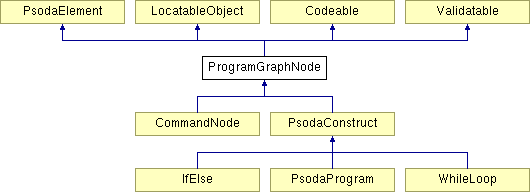
\includegraphics[width=.9\linewidth]{images/classProgramGraphNode.png}
    \end{center}
    \caption{The Hierarchy of a ProgramGraphNode}
  \end{figure}

  A PsodaProgram is a list of ProgramGraphNodes, each node being a simple command call (CommandNode) or a more complicated construction (PsodaConstruct) such as a loop or conditional.
  In order to build a nested program graph structure during a sequential parse of the input file, the PsodaProgram object keeps a build stack that allows new nodes to be opened, closed, or added.
  At any point, the top node of the stack can be referenced.
  In this way, information learned about the node currently being built is added to the correct node from different levels of the parser recursion.
  Such information includes the name of commands, parameters passed to commands, conditional expressions for loops and conditional statements, as well as entire command calls and nested constructs that should be added to the body of the current construct.

  \subsection{CommandNode}
  CommandNodes store the name of a command (regardless of its being built-in or user-defined) as well as the parameters which should be passed when the command is called.
  Also, it is in the CommandNode that much of the scoping and environment ``magic'' happens which we will discuss further in Section \ref{sec:scope}.
  When a command node is executed, the CommandNode uses the stored command name to retrieve the actual command definition from the interpreter.
  The parameters are then evaluated and the specific command is executed.

  \subsection{PsodaConstruct}
  The principal purpose of the creation of PsodaScript was to facilitate the scripting of meta-search algorithms from within the PSODA framework.
  Loop and Conditional constructs are the main mechanism for completing this task.
  There are currently three types of PsodaConstructs: PsodaProgram, IfElse, and WhileLoop.
  A PsodaProgram is executed by sequentially executing each ProgramGraphNode in its list of nodes.
  Since conditional and looping constructions contain complete internal program blocks which are executed as nested sub-programs, we take advantage of the PsodaProgram class to represent any block of PsodaScript code.

  An IfElse node simply contains a list of IfThenPair pointers.
  Each pair contains a pointer to an Expression that can be evaluated (more on this in Section \ref{sec:expressions}) as well as a corresponding PsodaProgram.
  With this data structure, we can construct a simple {\emph{if}} statement, add an arbitrary number of {\emph{elsif}} sections, and add a final {\emph{else}} section by setting the condition in the final IfThenPair to {\emph{true}}.
  During execution, the conditions are evaluated in sequence until a true condition is found at which point the program with execute the PsodaProgram associated with that condition.

  Similar to the if construct, the WhileLoop consists of a single Expression with a corresponding PsodaProgram loop body.
  The loop body is repeatedly executed until the expression evaluates to {\emph{false}}.
  If the expression evaluates to {\emph{false}} on the first iteration, the loop body is skipped without ever being executed.

  \section{Variables and Expressions}
  \label{sec:expressions}
  Adding variables and expressions to PsodaScript for use in the above mentioned constructs can be discussed under the following topics:

  \begin{enumerate}
    \item{Implementation of data structures for expressions}
    \item{Modification of the lexical analyzer and parser to recognize the given syntax}
    \item{Establishment of a structure and semantics for a variable environment including variable scoping}
    \item{Development of syntax and semantics for using and modifying variables}
  \end{enumerate}

  In this section I briefly discuss the issues and decisions involved in the first two of these tasks.
  Section \ref{sec:scope} will address the the remaining two tasks.

  \begin{figure}
    \label{fig:expression}
    \begin{center}
      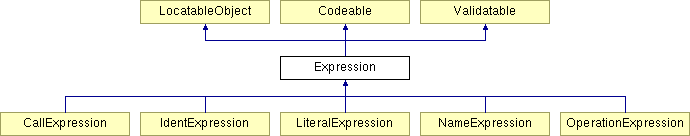
\includegraphics[width=.9\linewidth]{images/classExpression.png}
    \end{center}
    \caption{Expression Class Inheritance Hierarchy}
  \end{figure}

  \subsection{Implementing Expressions}

  Variables are used by programmers as a place to store information and as a tool in working with that information.
  There are five types of Expression as shown in Figure \ref{fig:expression}.
  
  The most basic expression is the LiteralExpression which hold a Literal value.
  Currently the following are the types of literal values in PsodaScript:

  \begin{itemize}
    \item{BoolLiteral---Boolean value}
    \item{IntLiteral---integer value}
    \item{StringLiteral---a character string}
    \item{TreeLiteral---a Phylogenetic Tree}
    \item{Data---holds a void pointer to C++ data}
    \item{UndefinedLiteral---contains no valid information}
  \end{itemize}
  
  An IdentExpression is used to refer to a variable and evaluates to the current value of the variable in the current environment.

  The CallExpression is used to call a command (whether built-in or user-defined) and evaluates to the return value of the called command.

  The NameExpression class was created to cope with a curiosity of PAUP* in which character strings are not enclosed in quotes when they are passed in as parameter values.
  Since an unquoted string may syntactically fit the description of both a variable reference as well as a string literal, the parser must create an expression object that can make a smart decision about how the expression should be interpreted at evaluation time.
  The NameExpression internally builds both types of expression and if evaluating the IdentExpression throws an UndefinedVariableException, the StringLiteralExpression is evaluated and its value is returned.

  An OperationExpression is created to perform operations on up to two sub-expressions.
  An OperationExpression contains up to two Expression pointers which serve as operands and a single Operator pointer which may be one of the following currently defined Operators:

  \begin{itemize}
    \item{NegationOp}
    \item{AdditionOp}
    \item{SubtractionOp}
    \item{MultiplicationOp}
    \item{DivisionOp}
    \item{ModOp---Modulus}
    \item{CatOp---Concatenation}
    \item{EqualityOp}
    \item{InequalityOp}
    \item{GreaterThanOp}
    \item{GreaterThanOrEqualOp}
    \item{LessThanOp}
    \item{LessThanOrEqualOp}
    \item{LogicalAndOp}
    \item{LogicalNotOp}
    \item{LogicalOrOp}
    \item{ParenthesesOp}
    \item{PostDecrOp---Postfix Decrement}
    \item{PostIncrOp---Postfix Increment}
    \item{PreDecrOp---Prefix Decrement}
    \item{PreIncrOp---Prefix Increment}
  \end{itemize}

  Any Operator class implements an operateOn() method that takes an environment and two (possibly null) expressions on which to operate and returns a reference to a Literal which it temporarily stores as the result of the operation.

  \subsection{Parsing Expressions}

  In addition to creating the structure and logic behind each of these expressions, literals, and operators, we also had to make some significant changes to the PSODA lexical analyzer and parser.
  The rules for the PSODA lexical analyzer are written in a special language used by the lexical analyzer generator, FLEX (Fast Lexical Analyzer Generator).
  Bison was used for creating the parser from a file containing a grammar definition mixed with C++ code to be executed as rules are recognized.

  \section{Variable Environment and Scoping}
  \label{sec:scope}

  PAUP* supports a feature that looks so much like variables that for a time we fooled ourselves into thinking that they were variables.
  The {\emph{set}} command found in PAUP*, and implemented in PSODA before the PsodaScript project began, facilitates setting a given parameter to a value that will be used in subsequent command calls until it is set to something else.
  Initially it seemed natural that the {\emph{set}} command would be the mechanism for updating variable values; however, we eventually realized that unexpected behavior could result if people began using already used parameter names as variables.
  Eventually, we saw that the {\emph{set}} command's role could be seen as setting default parameters for commands.
  To avoid unintended side effects from overloading the role of the {\emph{set}} command, we constructed a new syntax and intuitive semantics for variable assignments including well defined scoping rules.

  Variable environments keep track of variables that have been declared and the values that are currently assigned to those variables.
  The two principle methods on the Environment class are {\emph{set}} and {\emph{lookup}} which respectively set and return the value of a given variable.
  Environments may also extend a base environment which means that if a variable is not found in the current environment, the environment will look-up the value of the variable in its base environment.
  To avoid memory leaks, as variables in an environment are assigned literal values, the Environment class creates copies of the values on the heap and frees the memory as appropriate.

  When parameters are passed we had to decide how much of the current environment would continue to be visible during the execution of the command.
  PsodaScript uses a method of parameter passing commonly referred to as ``pass-by-value.''
  Parameters are evaluated to their current values and these values are placed in a new environment which extends the default environment for the command.
  Finally, a read-only environment is created on the stack which protects the default values from being changed.
  If a command tries to assign a value to a default variable, a new variable is created in the outermost scope of the running command.
  Program blocks, the body of loops, and conditional constructs each receive their own scope which extends the scope of the program at that point.

  \section{User-Defined Commands}
  User-defined commands allow script writers to wrap useful functionality into a new command---in a sense, extending PSODA without having to recompile or be familiar with the PSODA code-base.

  As with the other features that we were adding to the PSODA scripting framework, we wanted the addition of user-defined commands to be invisible to the beginning user.
  We were not satisfied with any addition that would pose incompatibilities with the existing syntax and semantics.
  User-defined commands are called as if they were built-in commands, and scoping and parameter passing for user-defined commands is also treated in the same way as for built-in commands.

  We developed a syntax for command declaration that was also easy to remember because commands are created with virtually the same syntax with which they are executed.
  When a command is defined, a list of default values is created which simultaneously tells the PsodaScript engine what parameters should be allowed to be set or passed for the command while also specifying the values that these variables should take should a caller fail to pass in a value for a recognized parameter.
 
  Because of this mechanism for specifying default values, parameters in user-defined commands are optional.
  Default parameter values for specific commands or for all commands can be changed during the program using the {\emph{set}} command.
  Because of default values, parameters are optional.

  Recursive command calls are also possible from within user-defined commands.
  Since a new environment is created on the stack when a command is executed, the run time stack keeps track of the depth of recursion and the values of the variables.

  \section{Error Checking}
  One of the major struggles in programming generally as well as in developing PsodaScript is identifying misunderstandings between the interpreter and whomever is writing the script.
  We found it necessary to significantly improve the error handling of the system---not only to make it more usable, but also to help us in development.
  To this purpose, we devised a mechanism for tracking the location of the objects that were parsed from the PSODA program block.
  Error messages can now print out the precise position, including the starting row and column and the ending row and column of the code in question.

  We devised several Exceptions that could be thrown by the parser or interpreter which would either issue warnings or display error messages and halt execution.
  We also developed a system for recursively printing out the complete program graph as it is generated by the parser.
  This was useful for debugging both PsodaScript programs as well as the PsodaScript engine itself.

  \chapter{Suggested Future Additions to PsodaScript}
  I include here a high level description of several features that I would recommend as future additions to PsodaScript.
 
  \section{The {\emph{reset}} and {\emph{get}} Commands}
  In a similar spirit to the {\emph{set}} command, the {\emph{reset}} command would take a list of parameter names and would reset the default values for those parameters to their initial default values, either for all commands or for a particular command (if the curly-brace notation is used).
  The {\emph{get}} command would similarly return the current default value of a given parameter.
  Typically, a specific command would be specified using curly braces; however, if no specific command is specified, the {\emph{get}} command would return a value if a global {\emph{set}} had been called for a parameter and {\emph{Undefined}} otherwise.

  \section{Fix the {\emph{execute}} Command}
  The execute command allows one to execute an external program with command-line arguments from within a PsodaScript program.
  Some further work needs to be done to make sure that this command behaves properly.

  \chapter{On A Personal Note}
  Aside from the potential benefits to the field of bioinformatics mentioned in the introduction, several personal motives influenced my decision to participate in this project. 
  As the winter semester of 2007 began, my goal to become a computer science professor had led me to seek out research opportunities.
  A new course was being offered that allowed interested undergraduate students to participate in a mentored research/capstone experience.
  Among the proposed projects was a proposal by the Computational Sciences Laboratory to develop an internal interpreted programming language for their open-source phylogenetic research package, PSODA.
  
  My love of language is perhaps one of the main reasons that computer science appeals to me.
  As we perform various tasks, we are exposed to a wide variety of programming and markup languages.
  A course in compilers and another about the essentials of programming languages had given me sufficient background for me to feel confident in my ability to successfully complete the project.
  I also persuaded myself that my fluency in Portuguese and interest in other natural languages would perhaps give some added insight to language decisions.
  
  I was also interested in the opportunity to contribute to an open-source project, something that I had often admired but never before done.
  Initially, I did not anticipate the project becoming my honors thesis nor did I realize the prospect of coauthoring and presenting at a conference a paper based on the work.
  Furthermore, although I didn't realize it at the time, this would also be the largest software project on which I had worked and my most significant investment of time to a single software project.

  \chapter{Conclusion}
  Our creation and implementation of the PsodaScript language within the PSODA framework provides phylogenetic researchers with a powerful tool in exploiting and exploring phylogenetic meta-searching.
  The project has served as a personal proving ground for many of the principles I have studied in the computer science curriculum and has served as a significant source of practical experience in software development.

  \appendix

  \chapter{The PsodaScript Language: A Primer}
  PsodaScript is an internal scripting language developed especially for the PSODA framework.
  Specifically, PsodaScript aims to provide enhanced meta-search capabilities inside of the PSODA package.
  This manual describes the syntax and semantics of the PsodaScript language.

  \subsection{Built-in Commands and Parameters}
  The basic building block of a PsodaScript program is the {\em Command}.
  A Command is issued (or called) to perform a given action.
  For instance, the {\emph{hsearch}} command performs a heuristic search, the {\emph{gettrees}} command loads phylogenetic trees from a file into the tree repository, the {\emph{print}} command prints text to the console, and the {\emph{set}} command sets parameter defaults.
  Table \ref{tab:commands} lists several of the built-in commands available in PsodaScript.
  Table \ref{tab:functions} lists several built-in commands which are called ``functions'' because they have return values.
  
  \begin{table}\centering
    \ras{1.3}
    \begin{tabular}{@{}lp{60ex}@{}}\toprule
      Command Name              &       Description \\ \midrule
      Align                     &	Aligns the current data-set \\
      BackupRepository   	&	Stores the trees in the current repository into a backup repository \\
      Break     		&	Breaks out of the innermost while loop construct \\
      CombineRepositories	&	Combines the trees from the backup and current repository \\
      GetTrees   		&	Load the tree repository with trees from a file  \\
      Graph     		&	Turns on or off the graphical plotting mechanism \\
      HSearch		     	&	Perform a heuristic search  \\
      Print		     	&	Prints text to the console \\
      PScores		     	&	Scores trees in the repository using parsimony \\
      Quit			&	Terminates the current PsodaScript program \\
      RandomMorph		&	Randomly morphs the trees in the repository \\
      RAxMLSearch		&	Performs a search using RAxML \\
      SaveTrees		     	&	Saves the trees in the repository to a specified file \\
      Set			&	Sets the default value for specified parameters \\
      SRandom		     	&	Seeds the random number generator \\
      Weights		     	&	Sets the weights to the sequence data columns \\
    \end{tabular}
    \label{tab:commands}
    \caption{Some Built-In PsodaScript Commands}
  \end{table}

  \begin{table}\centering
    \ras{1.3}
    \begin{tabular}{@{}lp{60ex}@{}}\toprule
      Command Name              &       Description \\ \midrule
      GetBestScore	     	&	Returns the score of the best tree in the repository \\
      GetNumChars	     	&	Returns the number of columns in the current data-set \\
      Random		     	&	Returns a random integer greater than or equal to 0 and less than the number passed in \\
      Time                   	&	Returns the current time in seconds\\ \bottomrule
    \end{tabular}
    \label{tab:functions}
    \caption{Some Built-In PsodaScript Functions}
  \end{table}

  The syntax used to issue most commands consists of the command name followed by a (possibly empty) list of parameters and terminated with a semicolon.
  Sample \ref{code:command} shows several examples of valid command calls.
  
  \begin{code}
    \caption{PsodaScript Command Syntax}
    \label{code:command}
    \small
    \vspace{10pt}
    \begin{verbatim}
      hsearch nreps=5 start=current;
      hsearch (nreps=5 start=current);
      hsearch (nreps=5, start=current);
      hsearch nreps=5, start=current;
      hsearch;
      hsearch();

      quit warntosave;
      quit warntosave=yes;
    \end{verbatim}
  \end{code}

  Parameters allow the user to specify certain specifics of what a command should do.
  Each command recognizes some set of parameter names which are used to specify how the command should behave.
  For each parameter that a given command recognizes, the command has a default value that will be used for that parameter if no other value is passed in via the parameter list. 
  The parameter list consists of 0 or more parameter {\emph{name}}={\emph{value}} pairs which may optionally be separated by commas.
  The parameter list may also optionally be enclosed in parentheses.
  Listing a parameter name in the parameter list without specifying a value effectively passes the string ``yes'' as the value of the parameter.
  Parameter values may be variables, integers, or character strings enclosed in double-quotes.

  \subsubsection{Special Commands}
  \label{sec:specialcommands}

  The {\emph{set}} command can be used to set the defaults used for given parameters.
  For instance, \verb|set nreps=10 iterations=5;| sets the default value for the {\emph{nreps}} parameter to be 10 and that of {\emph{iterations}} to be 5.

  The {\emph{set}} command can be performed on a specific command by preceding the command list with a command name enclosed in curly braces.
  For example, \verb|set{hsearch} nreps=10 iterations=10;| sets the {\emph{nreps}} and {\emph{iterations}} default values for the {\emph{hsearch}} command only.

  \section{The {\emph{source}} Command}
  The built-in {\emph{source}} command takes the name of a file as the ``file'' parameter parses that file and runs the the resulting program graph, registering any user-defined commands with the interpreter as they are found.

  \section{The {\emph{loaddata}} Command}
  The built-in {\emph{loaddata}} is complementary to the {\emph{source}} command.  While {\emph{source}} only runs the program block of the file, {\emph{loaddata}} only interprets the first data block that is found in the given file.  By default the command sets the loaded data as the current dataset.

  \subsection{Variables}
  Variables are similar to parameters in that they are names which reference values.
  However, parameters are used to pass information and settings into a command---the names of accepted parameters having been determined by the creator of the command---while variables are a way for a person writing in PsodaScript to store and work with data, deciding how to name and use the variables he creates.
  They are called ``variables'' because the value stored in a variable can be replaced by a different value later in the program.
  Consider the statement \verb|x = 5;|
  If the variable $x$ exists in the given scope (more on scope in Section \ref{sec:variablescope}), it is updated to hold the value \verb|5|, otherwise a new variable $x$ is created in the current scope and initialized with the value 5.
  Variables can be passed into commands via command parameters just as literal values are passed.
  Variables may also be combined into expressions using operators (see section \ref{sec:operators}).
  
  \subsection{Data Types}
  Any variable can be assigned any valid data type.
  Even though a given variable can hold any valid piece of data---regardless of the type of the variable and the type of the data, variables are weakly typed because certain operations only make sense on certain data types.
  Variables may store the following types of data:
  \begin{enumerate}
  \item{Integer numbers}
%  \item{Floating point numbers} [We need to add this]
  \item{Character Strings---``myString''}
  \end{enumerate}
  Future data types may include floating point numbers, phylogenetic trees, tree repositories, and arrays.

  \subsection{Expressions \& Operators}
  \label{sec:operators}
  Expressions are segments of PsodaScript code that can be evaluated to some literal value.
  For example, when an assignment is made, the code segment on the right-hand side of the equals sign is evaluated as an expression and the variable is assigned the resulting value.
  Parameter values are also expressions.
  Each time a command is executed, each expression in the parameter list is evaluated and the results are passed in as the values of the given parameters.

  There are essentially four types of expressions:
  \begin{enumerate}
  \item{A literal value (e.g. \verb|count = 10;|).}
  \item{A variable (e.g. \verb|tempCount = count;|) {\em if count has not been initialized in the current scope, the expression \verb|count| will evaluate to the string ``count''}.}
  \item{A call to a command that returns a value (e.g. \verb|randomNum = random (max = 10);| \emph{note: parentheses are required around the parameter list (even if it is empty) if the return value of the command is being used as part of an expression}.}
  \item{An expression composed of smaller sub-expressions using expression operators.}
  \end{enumerate}
  
%  --We need to put in the exponent operator--
  
  If a variable is used in an expression and if that variable has not been initialized in the current scope, the variable expression will evaluate to a string containing the name of the variable (this was done for compatibility reasons with PAUP*).

  Some commands---such as the \verb|random| command return a value.
  These commands are often referred to as functions.
  Function calls may be made in expressions just as literal values are used.
  As described above, when function calls are used in expressions, the parameter list must always be surrounded by parentheses to avoid ambiguity.
  
  Expression operators follow conventional operator precedence.
  Table \ref{tab:operators} shows available operators listed in order of precedence (top-to-bottom) with the highest precedence at the top.
  Operators with equal precedence are grouped together in the table and are evaluated in order left to right, except in the case of the unary integer negation and logical not operators which cannot be used next consecutively.
  
  \begin{table}\centering
    \ras{1.3}
    \begin{tabular}{@{}ll@{}}\toprule
      Symbols & Description \\ \midrule
      () & Parentheses \\ \midrule
      \verb|++| & Increment \\
      \verb|--| & Decrement \\ \midrule
      \verb|-| & Unary Integer Negation \\
      \verb|!| & Logical Not \\ \midrule
      \verb|*| & Multiplication \\
      \verb|/| & Division \\
      \verb|%| & Modulus \\ \midrule
      \verb|+| & Addition \\
      \verb|-| & Subtraction \\ \midrule
      \verb|.| & String Concatenation \\ \midrule
      \verb|<| & Less Than \\
      \verb|<=| & Less Than or Equal \\
      \verb|>=| & Greater Than or Equal \\
      \verb|>| & Greater Than \\ \midrule
      \verb|==| & Equal \\
      \verb|!=| & Not Equal \\ \midrule
      \verb|&&| & Logical And \\ \midrule
      \verb!||! & Logical Or \\ \bottomrule
    \end{tabular}
    \label{tab:operators}
    \caption{PsodaScript Operators}
  \end{table}

  \subsection{Loops \& Conditionals}
  Looping and conditional constructs allow users to control the flow of the program based on its current state.

  \subsubsection{The While Loop}
  A While loop is used when a programmer wants to repeat a block of code as long as a certain condition holds.
  The PsodaScript {\em while} construct consists of a conditional expression and a loop body which is made up of 0 or more lines of PsodaScript code.
  Sample \ref{code:while} illustrates a simple While Loop.

% [Case sensitivity]

  \begin{code}
    \caption{While Loop Syntax}
    \label{code:while}
    \small
    \vspace{10pt}
    \begin{verbatim}
  count = 0;
  while (count < 10)
    count++;
    print (count);
  endwhile;
    \end{verbatim}
  \end{code}

  In Sample \ref{code:while}, after the variable $count$ is initialized to 0, the condition \verb|count < 10| is evaluated before each iteration of the loop.
  If the condition evaluates to {\em false}, the body of the loop is skipped and the program continues from that point (after the \verb|endwhile;|).
  If the condition evaluates to {\em true}, the body of the loop is executed and the process is repeated until the condition no longer evaluates to {\emph{true}}.
  The output of Sample \ref{code:while} would be the numbers 0 through 9 being printed to the console:

  \begin{verbatim}
0123456789
  \end{verbatim}

  \subsubsection{The {\emph{break}} command}
  The break command is a special command that takes no parameters and causes the program to break out of the innermost While Loop and continue at the end of the loop.
  Sample \ref{code:break} uses the break command to show an alternative loop that is equivalent to that in Sample \ref{code:while}.

  \begin{code}
    \caption{The {\emph{break}} Command}
    \label{code:break}
    \small
    \vspace{10pt}
    \begin{verbatim}
  count = 0;
  while (true)
    if (count >= 10)
      break;
    endif;

    count++;
    print (count);
  endwhile;
    \end{verbatim}
  \end{code}

  \subsubsection{Using the {\emph{if}} Construct}
  In PsodaScript, conditional constructs are used to select a group of actions to execute based on the evaluation of some condition.
  Conditional statements in English are of the form ``if $condition$ then $consequence$.''
  Sample \ref{code:if} shows the syntax of a simple {\em if} construct in PsodaScript.

  \begin{code}
    \caption{The {\emph{if}} Syntax}
    \label{code:if}
    \small
    \vspace{10pt}
    \begin{verbatim}
  count = 5;
  if (count < 10)
    print ("Count is less than 10");
  endif;
    \end{verbatim}
  \end{code}

  Since $count$ is assigned the value 5, the condition in Sample \ref{code:if} will evaluate to {\emph{true}} and the body of the conditional will be executed, printing the string ``\verb|Count is less than 10|'' to the console.

%  [we need to change to else if]

  \subsubsection{Using the {\emph{elsif}} keyword}
  The {\emph{elsif}} keyword allows the user to specify alternative blocks of code to execute based on alternative conditions.
%  [let's make true be anything greater than 0]
  The program will execute the block of code following the first condition that evaluates to {\em true}.
  After executing the block of code, the program breaks out of the {\em if} construct and continues execution (after the \verb|endif;| statement).

  \begin{code}
    \caption{The {\emph{elsif}} Syntax}
    \label{code:elsif}
    \small
    \vspace{10pt}
    \begin{verbatim}
  count = 15;
  if (count < 10)
    print ("Count is less than 10");
  elsif (count < 15)
    print ("Count is between 10 and 15");
  elsif (count < 25)
    print ("Count is between 15 and 25");
  endif;
    \end{verbatim}
  \end{code}
  
  In Sample \ref{code:elsif}, since $count$ is set to 15, the first two conditions fail, but \verb|count < 25| evaluates to {\emph{true}} and the text ``\verb|Count is between 15 and 25|'' is printed.

  \subsubsection{Using the {\emph{else}} keyword}
  The {\emph{else}} keyword can be used to specify an alternative block of code to be executed if all previous conditions fail.
  Consider in Sample \ref{code:else}.
  Since $count$ is set to 15, the condition \verb|count < 10| evaluates to {\emph{false}} so the following body is not executed.
  Instead, the body following the {\emph{else}} keyword is executed and the text ``\verb|Count is not less than 10|'' is printed to the screen.

  \begin{code}
    \caption{The {\emph{else}} Syntax}
    \label{code:else}
    \small
    \vspace{10pt}
    \begin{verbatim}
  count = 15;
  if (count < 10)
    print ("Count is less than 10");
  elsif (count < 15)
    print ("Count is between 10 and 15");
  elsif (count < 25)
    print ("Count is between 15 and 25");
  else
    print ("Count is greater than or equal to 25");
  endif;
    \end{verbatim}
  \end{code}

  \subsection{User-Defined Commands}
  PsodaScript allows users to write and use their own commands as if they were part of the PsodaScript language.
  This is useful for many reasons.
  As a program becomes more complicated, it is often helpful to divide the program into smaller parts that can be programmed separately.
  Frequently a meta-search will include several similar series of commands that could be factored out into a user-defined command.
  
%  [      Key words (like ``begin'') are case-insensitive]

  A user-defined command represents a self contained PsodaScript program.
  Sample \ref{code:user-defined-command} demonstrates the syntax for defining a simple user-defined command.
  First, the key word \verb|begin| is used, followed by the command name and a list of parameter defaults.
  This parameter defaults list tells PsodaScript what parameters may be passed into your command as well as the initial default values to be used if any parameters are missing from the parameter list when the command is called.

  \begin{code}
    \caption{User-defined Command Syntax}
    \label{code:user-defined-command}
    \small
    \vspace{10pt}
    \begin{verbatim}
  begin myCommand param1 = 5 param2 = 10;
    print ("This is my own command\n");
    print ("param1 = " . param1 . "\n");
    print ("param2 = " . param2 . "\n");
    hsearch;
  end;
    \end{verbatim}
  \end{code}

  Since the parameter defaults list follows the same syntax as the parameter list in a command call statement, the three variations shown in Sample \ref{code:user-defined-command2} are also valid and equivalent to the code in Sample \ref{code:user-defined-command}.
  
  \begin{code}
    \caption{More User-defined Command Syntax}
    \label{code:user-defined-command2}
    \small
    \vspace{10pt}
    \begin{verbatim}
  begin myCommand (param1=5, param2=10);
    [command body]
  end;

  begin myCommand(param1 = 5, param2 = 10);
    [command body]
  end;

  begin myCommand (param1 = 5 param2 = 10);
    [command body]
  end;
    \end{verbatim}
  \end{code}

  \subsubsection{The {\emph{return}} statement}
  The return command is similar to the break command.
  It breaks out of the current user-defined command body and returns the value passed by the \verb|value| parameter. 
  If the user-defined command was called from an expression such as in \verb|myVar = myCommand();|, the call expression evaluates to the value of the \verb|value| parameter in the return command that is executed.
  Multiple return commands may appear in the same user-defined command; however, at most one will be executed during a given call to the user-defined command.
  If the flow reaches the end of the user-defined command without encountering a return command, a special value ({\em Undefined}) is returned.
  Sample \ref{code:return} shows an example of a user-defined command using a return statement.
%  [When are parentheses needed around expressions (for instance in parameter values)]

  \begin{code}
    \caption{The {\emph{return}} Command}
    \label{code:return}
    \small
    \vspace{10pt}
    \begin{verbatim}
  begin multiply (a = 1, b = 1);
    print ("a = " . a . "\t");
    print ("b = " . b . "\n");
    return (a*b);
  end;
  
  myProduct = multiply(a = 10 b = 35);
  print (myProduct);
    \end{verbatim}
  \end{code}


  \subsubsection{Recursion in PsodaScript}
  PsodaScript user-defined commands support recursive calls.
  This means that a function can call itself (presumably with different parameter values) in order to eventually arrive at the correct solution.
  It is important to keep the following points in mind when making recursive functions:
  \begin{enumerate}
    \item{There must be a base condition for which case no recursive call is made}
    \item{Each recursive call must bring the function closer to the base condition}
  \end{enumerate}

  Sample \ref{code:recursion} in Appendix \ref{sec:code} demonstrates the use of a recursive command call to calculate (albeit inefficiently) the first several numbers of the Fibonacci sequence.

  \subsubsection{Pass-by-Reference}
  Perhaps the most intuitive form of passing parameters is what is known as ``pass-by-value'' which means that the value of the parameter is copied into the variable of the same name for the body of the user-defined command.
  When parameters are passed by value, changing the variable inside of the user-defined command has no effect on the parameter that was passed in.
  
  Passing by reference simply means that the variable used (and potentially modified) within a user-defined command will be the actual variable that was passed in rather than a new variable initialized to the same value.
  This can be useful in many ways:
  
  \begin{enumerate}
  \item{It can avoid copying values of large variables}
  \item{It can be used to change the values of variables stored outside of the user-defined command}
  \item{It can be used to return more than one value from a command}
  \item{It can be used to return optional return values}
  \end{enumerate}
  
  If a variable is to be passed by reference, this will be represented in the command definition by placing an ampersand after the name of the parameter.
  Parameters that are designated to be received by reference do not need to have a default value specified (as do other parameters).
  If a pass-by-reference paramter is not given a default value, a valid variable will need to be passed by the caller.
  If a default value is specified and a variable is not passed by reference as the parameter, a new local variable will be created and assigned the default value.

  To illustrate, in the user-defined command shown in Sample \ref{code:pass-by-reference}, the parameter {\emph{best\_score}} is declared to be passed by reference.
  If a valid variable is not passed as the {\emph{best\_score}} parameter, PsodaScript should issue an error.
  The parameter {\emph{counter}}, on the other hand, is also passed by reference, but the syntax specifies that if the parameter is not given, a temporary variable with the name {\emph{counter}}, will be created and initialized to 0.
  This is useful for allowing multiple optional return values.
  If the caller is not interested in knowing the value of the counter after {\emph{myRatchet}} is run, it would not need pass in a variable for {\emph{counter}}.
  If a {\emph{counter}} parameter is passed but is not a valid variable (e.g. if the value 5 were passed rather than a variable name), an error should still be issued. (The errors are not necessarily being issued right now).
  
  \begin{code}
    \caption{Passing-by-Reference Syntax}
    \label{code:pass-by-reference}
    \small
    \vspace{10pt}
    \begin{verbatim}
begin myRatchet (percent_to_skew=45, range=15,
                 best_score&, counter&=0);
  [body of myRatchet]
end;
    \end{verbatim}
  \end{code}

  \subsubsection{Inline User-Defined Commands}
  By placing an asterisk after the {\emph{begin}} keyword of a command definition, you can tell the interpreter to give the called function a read only copy of all variables visible to the caller of the command (however, references passed to the command work as normal).

  \subsection{Variable Scope}
  \label{sec:variablescope}

  Section \ref{sec:specialcommands} presented the {\emph{set}} command which is used to set parameter default values.
  A difference between variables and parameters is that variables are created in a specific scope while setting a parameter default effects all command calls regardless of where the command call is made.
  A scope represents a portion of code in which a variable is ``visible,''---that is, defined.
  Scope helps to keep separate pieces of PsodaScript independent.
  For instance, a variable created inside of a user-defined command will not be visible outside of the command, and will not, therefore, affect nor be modified by other parts of the program.
  The body of a user-defined command and a while loop, as well as the bodies of an if/else construct, each create a new, nested inner scope.
%  [we could not allow (var) --- like java]
  Scopes are nested in the sense that variables in an outer scope are visible to the inner scope but not vice-versa.

  \begin{code}
    \caption{Variable Scope}
    \label{code:scope}
    \small
    \vspace{10pt}
    \begin{verbatim}
#NEXUS
BEGIN PSODA;

  outerCounter = 0;

  print "Before Loop\n";
  print "Ounter Counter: " . outerCounter . "\n";
  print "Inner Counter: " . innerCounter . "\n";

  print "\tIn Loop\n";
  while (outerCounter < 5)
    outerCounter++;
    print "\tInner Counter (undefined): " . innerCounter . "\n";
    innerCounter = outerCounter;
    print "\tOuter Counter: " . outerCounter . "\n";
    print "\tInner Counter (defined): " . innerCounter . "\n";
  endwhile;

  print "Done with loop\n";
  print "Outer Counter: " . outerCounter . "\n";
  print "Inner Counter: " . innerCounter . "\n";

END;
    \end{verbatim}
  \end{code}
  
  Consider Sample \ref{code:scope}.
  Before the loop, {\emph{outerCounter}} is declared and initialized to 0 but {\emph{innerCounter}} is undefined.
  In each iteration of the loop {\emph{innerCounter}} is created in that inner loop and assigned the value of {\emph{outerCounter}} until the end of the inner code block, at which point the variable {\emph{innerCounter}} goes out of scope.
  Since {\emph{outerCounter}} was declared in the outer scope, its value persists and is incremented on each iteration of the loop.

  \chapter{Sample PsodaScript Applications}
  \label{sec:code}

  To demonstrate the capabilities of PsodaScript, I include here a few sample applications.
  The first example is a simple demonstration of recursion in PsodaScript.
  The second example is a possible application of the Ratchet in PsodaScript.
  I also include an adaptation of the ratchet.
%  Finally, I include an application which uses looping to give feedback to the sequence alignment process.

  \section{Recursive Fibonacci Sequence}
  \label{code:recursion}
  \begin{singlespace}
  \begin{verbatim}
#NEXUS
BEGIN PSODA;

begin fibinacci(index = 1);
  fibNumber = "*";
  if (index >= 0)
    if (index == 0 || index == 1)
      fibNumber = 1;
    else
      fibNumber = fibinacci(index = (index - 1))
                + fibinacci(index = (index - 2));
    endif;
  endif;
  return fibNumber;
end;

i = 0;
while (i < 20)
  print fibinacci(index = i) . endl;
  i++;
endwhile;

END;
  \end{verbatim}
  \end{singlespace}
  \section{The Ratchet in PsodaScript}
  \label{code:ratchet}
  \begin{singlespace}
  \begin{verbatim}
#NEXUS
[ load the data here ]

BEGIN PSODA;

begin randomReweight (range=3, percent=25);
  numColumns = getWeightsLength();
  numToChange = numColumns * percent / 100;
  j = 0;
  while (j < numToChange)
    column = random (max=numColumns) + 1;
    newWeight = random (max=range);
    weights newWeight:column;
    j++;
  endWhile;
end;

set (maxtrees=1, criterion=parsimony);
hsearch (start=stepwise, swap=tbr);
while (true)
  randomReweight (percent=20);
  hsearch (start=current, swap=tbr);
  weights reset;
  hsearch (start=current, swap=tbr);
  print ("Score: ");
  print (getBestScore() . endline);
endwhile;

END;
  \end{verbatim}
  \end{singlespace}
  
  \section{A Modified Ratchet}
  \label{code:modratchet}
  \begin{singlespace}
    \begin{verbatim}
#NEXUS
[ load the data here ]


BEGIN PSODA;

[
  Randomly skew a portion of the column weights

  @param int range   The new weight will be chosen withing the range of
                     0 to range - 1
  @param int percent About this many out of every 100 columns will be
                     randomly selected to be skewed
]
begin randomReweight (range=3, percent=25);
  numColumns = getNumChars();
  numToChange = numColumns * percent / 100;
  j = 0;
  while (j < numToChange)
    column = random (max=numColumns) + 1;
    newWeight = random (max=range);
    weights newWeight:column;
    j++;
  endWhile;
end;

[
  Format the time (given in seconds) as hours:minutes:seconds

  @param int time  The time in seconds to be formatted
  @return string   The formatted time
]
begin formatTime(time = 0);
  $time = time;
  $seconds = $time % 60;
  $time = $time - $seconds;
  $time = $time / 60;
  $minutes = $time % 60;
  $time = $time / 60;
  $hours = $time;
  $text = $hours . ":" . $minutes . ":" . $seconds;
  return $text;
end;

[
  Saves out the current trees in the repository with a name
  corresponding to the best score

  @return string  The name of the file to which the trees were saved
]
begin saveBestTrees();
    $score = getBestScore();
    $filename = "ratchetTree-" . $score . ".tre";
    savetrees (file = $filename);
    return $filename;
end;

[
  Main Program -- Performs the parsimony ratchet by continually skewing
  and resetting the column weights, saving out the trees when a lower score
  is found and printing out time and iteration information
]
startTime = time();
numIterations = 0;
set (maxtrees=1, criterion=parsimony);

[ Run an initial heuristic search and save out the trees. ]
hsearch (start=stepwise, swap=tbr);
saveBestTrees;
bestSoFar = getBestScore();
timeOfLastBest = time();
iterationsOfLastBest = numIterations;

while (true)

  [ Skew the weights, and run a search in the warped space. ]
  randomReweight (percent=20);
  hsearch (start=current, swap=tbr);

  [ Reset the weights, and run a real search. ]
  weights reset;
  hsearch (start=current, swap=tbr);
  numIterations++;

  thisScore = getBestScore();
  curTime = time();

  [
    If we found a new low score, save out the trees,
    print out the news, and update our info.
  ]
  if (thisScore < bestSoFar)
    bestSoFar = thisScore;
    message = "*Found new best score: " . bestSoFar . endline
      . "*Saved trees to: " . saveBestTrees() . endline;
    print (message);
    timeOfLastBest = curTime;
    iterationsOfLastBest = numIterations;
  endif;

  [ Print out a status message. ]
  message = "*Score So Far:\t" . bestSoFar
    . "\tTime:\t" . formatTime(time = (curTime - startTime))
    . "\tIteration:\t" . numIterations
    . "\tTime since last best:\t" . formatTime(time = (curTime - timeOfLastBest))
    . "\tIterations since last best:\t" . (numIterations - iterationsOfLastBest)
    . endline;
  print (message);

endwhile;

END;
    \end{verbatim}
  \end{singlespace}

  \backmatter

  \bibliographystyle{plain}
  
  \bibliography{honors_thesis}
\end{document}
